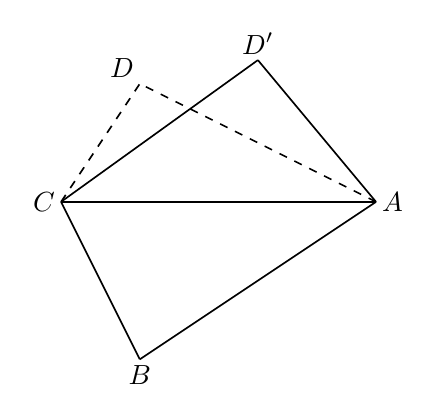
\begin{tikzpicture}[x=1cm,y=1cm,font=\normalsize,
  geometry edge/.style={solid,line width=.6pt},
  geometry label/.style={font=\normalsize,inner sep=2pt}]
\coordinate (C) at (0,2.0);
\coordinate (A) at (4,2.0);
\coordinate (B) at (1,0);
\coordinate (D) at (1,3.5);
\coordinate (Dp) at (2.5,3.8);
\draw[geometry edge] (C)--(A);
\draw[geometry edge] (C)--(B);
\draw[geometry edge] (A)--(B);
\draw[geometry edge] (C)--(Dp);
\draw[geometry edge] (A)--(Dp);
\draw[geometry edge,dashed] (C)--(D);
\draw[geometry edge,dashed] (A)--(D);
\node[geometry label,left] at (C) {$C$};
\node[geometry label,right] at (A) {$A$};
\node[geometry label,below] at (B) {$B$};
\node[geometry label,above left] at (D) {$D$};
\node[geometry label,above] at (Dp) {$D'$};
\end{tikzpicture}